% ----------------------------------------------------------------
%           Reforestation Logistic Transport Optimization
%
%                      Juan José H. Beltrán
%                    Kevin Martínez Trinidad
%                     Jesús Ramirez Mendieta
%                      Kaleb Flores Alfonso
% ----------------------------------------------------------------
\documentclass{amsart}
\usepackage{graphicx}
\usepackage[margin=3cm]{geometry}

% Para bibliografía
\usepackage[spanish]{babel}
\usepackage[babel]{csquotes}
\usepackage[backend=biber, style=apa]{biblatex}
\DeclareLanguageMapping{spanish}{spanish-apa}
\bibliography{sources/references.bib}

% Estilos de URL
\usepackage{hyperref}
\hypersetup{
    colorlinks=true,
    linkcolor=magenta,
    filecolor=magenta,      
    urlcolor=cyan,
    pdftitle={Overleaf Example},
    pdfpagemode=FullScreen,
    }
\urlstyle{same}


\begin{document}

% ---------------------------------- Portada ----------------------------------
    \begin{center}
        {\bfseries\LARGE Instituto Tecnológico de Monterrey\par}
        %\vspace{0.5cm}
        {\scshape\Large Escuela de Ingeniería y Ciencias\par}
        \vspace{0.5cm}
        {\scshape\Huge Reforestation Logistic Transport Optimization\par}
        \vspace{0.5cm}
        {Juan José H. Beltrán, Kevin Martínez Trinidad, Jesús Ramirez Mendieta, Kaleb Flores Alfonso\par}
        \vspace{0.5cm}
        {October, 2024}
        \vspace{0.5cm}
        
        \rule{15.5cm}{0.1pt}
    \end{center}


    % -------------------------------------- ENTREGA 1 --------------------------------------

    \section{Introduction}
    According to data from Comisión Nacional Forestal, using an internationally approved methodology with Sistema Satelital de Monitoreo Forestal (SAMOF), which photointerprets satellite images, on average, Mexico has demonstrated an annual deforestation rate of approximately 208,850 hectares per year during the period 2001—2019, which represents 0.31\% of the wooded forest area nationwide. In 2020, it was concluded that the main source of deforestation is the felling of trees for agriculture and illegal logging, accounting for 80\% of tropical deforestation \parencite{refForestal}.

    Deforestation directly affects the water cycle by reducing the capacity of forests to capture and regulate water flow, aggravating droughts and water scarcity for human consumption, industry and agriculture. Furthermore, forests are important for aquifer recharge and flood prevention.

    Biodiversity is also affected by destroying natural habitats and releasing large amounts of carbon stored in trees. Additionally, climate regulation and erosion prevention are lost. It has been estimated that deforestation is responsible for approximately 10\% of global greenhouse gas emissions.

    In response, the Government of Mexico together with SEMARNAT and its agencies have initiated strategies around prevention, inspection and verification, intelligence, judicialization of cases, social support and review of the legal framework to combat deforestation and illegal logging. Likewise, to contribute to the restoration of ecosystems, the choice of species for reforestation is based on criteria such as adaptability to the local climate, diversity and ecological benefits. Species distribution is planned considering site conditions and restoration objectives.

        \subsection{Problem Justification}
        Climate change and droughts are becoming important problems, not only for keeping ecosystems in harmony, but also for human activities.

        Deforestation is one of the main causes of droughts, in addition to accelerating climate change. In our country, deforestation is a bigger problem than is believed, as it is often carried out illegally or irresponsibly.

        Reforestation programs permit to reduce the negative effects of deforestation. Organizations like CONAFOR receive a limited amount of resources and have a maximum period of a few months a year to carry out reforestation.

        Consequently, a model that indicates which are the optimal routes and the appropriate time to carry them out, thus reducing the time and economic expense of the activity, is necessary to increase as much as possible the probabilities of successfully completing the project, using the least amount of resources possible.


        \subsection{Objective}
        The objective is to minimize both the distance, and consequently time, consumed by the trucks that transport the plants to the planting site. To do this, it is proposed to build a work plan that contains ordered routes that allow them to make all deliveries in the shortest time possible.

        \subsection{{Related Work}}

            \subsubsection{Flora in the Mexican Altiplano}
            The Mexican highlands is a term that refers to the area that extends from the border of Mexico with the United States to the approximate latitude of Mexico City, covering states such as Chihuahua, Coahuila, Nuevo León, Durango, San Luis Potosí, Jalisco, Puebla, among others (\cite{Lifeder}).
            In the southern part of the Mexican highlands it is common to find coniferous forests, in which it is possible to find species such as pines, ceiba, fir and holm oak, as well as occasional grasses (\cite{Lifeder}).
            \begin{itemize}
                \item Pines: Trees characteristic of the evergreen forest, which generally measure 15 to 45m (\cite{Masats}).
                \item Ceiba: They are very large trees, with deciduous leaves, with cultural and historical value. They usually measure 20 to 40 meters (\cite{Anónimo3}).
                \item Oyamel: It is a large evergreen tree, 25 to 30m high and 70 to 90cm in diameter. Species considered in danger of extinction mainly due to human activities, since it is used as fuel and firewood (\cite{Anónimo4}).
                \item Holm Oak: It has a large crown, with a rounded shape, and leafy leaves, which make it good for providing shade. It can measure up to 25m in height and has a wide and thick trunk (\cite{Aquae}).
            \end{itemize}

            On the other hand, in the dry zone of the high plateau the predominating species are the following (\cite{Lifeder}):
            \begin{itemize}
                \item Cactus: The characteristic inhabitant of the desert, they are characterized by storing large amounts of water that allows them to survive great droughts (\cite{Hernández}).
                \item Maguey: It contributes to the conservation and retention of the soil, at the same time that its juice allows the production of alcoholic beverages and is used for medicinal purposes (\cite{Hernández}).
                \item Ocotillo: Similar to the cactus, it is a thorny tree that requires little water to survive (\cite{Hernández}).
                \item Mezquite: They are deciduous trees that can measure 6 to 9 meters, they are characterized by the properties of their wood, which is widely used for cooking food (\cite{Anónimo5}).
             \end{itemize}

            \subsubsection{Tresbolillo Plantation Frame}
            In agriculture, it is well known that all plants require some space to grow and develop properly. This condition gives rise to the planting frames: the spatial arrangement and distance that exists between the plants. Each crop has a recommended planting framework, since its appropriate choice will favor lighting, light and nutrients; and will reduce the risk of pests and the spread of diseases (\cite{Balam2022}). There is a great variety of planting frames (Figure~\ref{fig:MarcosDePlantación}), such as square, rectangular, five gold, and staggered, just to mention a few (\cite{Balam2022}).
            
            \begin{figure}
                \centering
                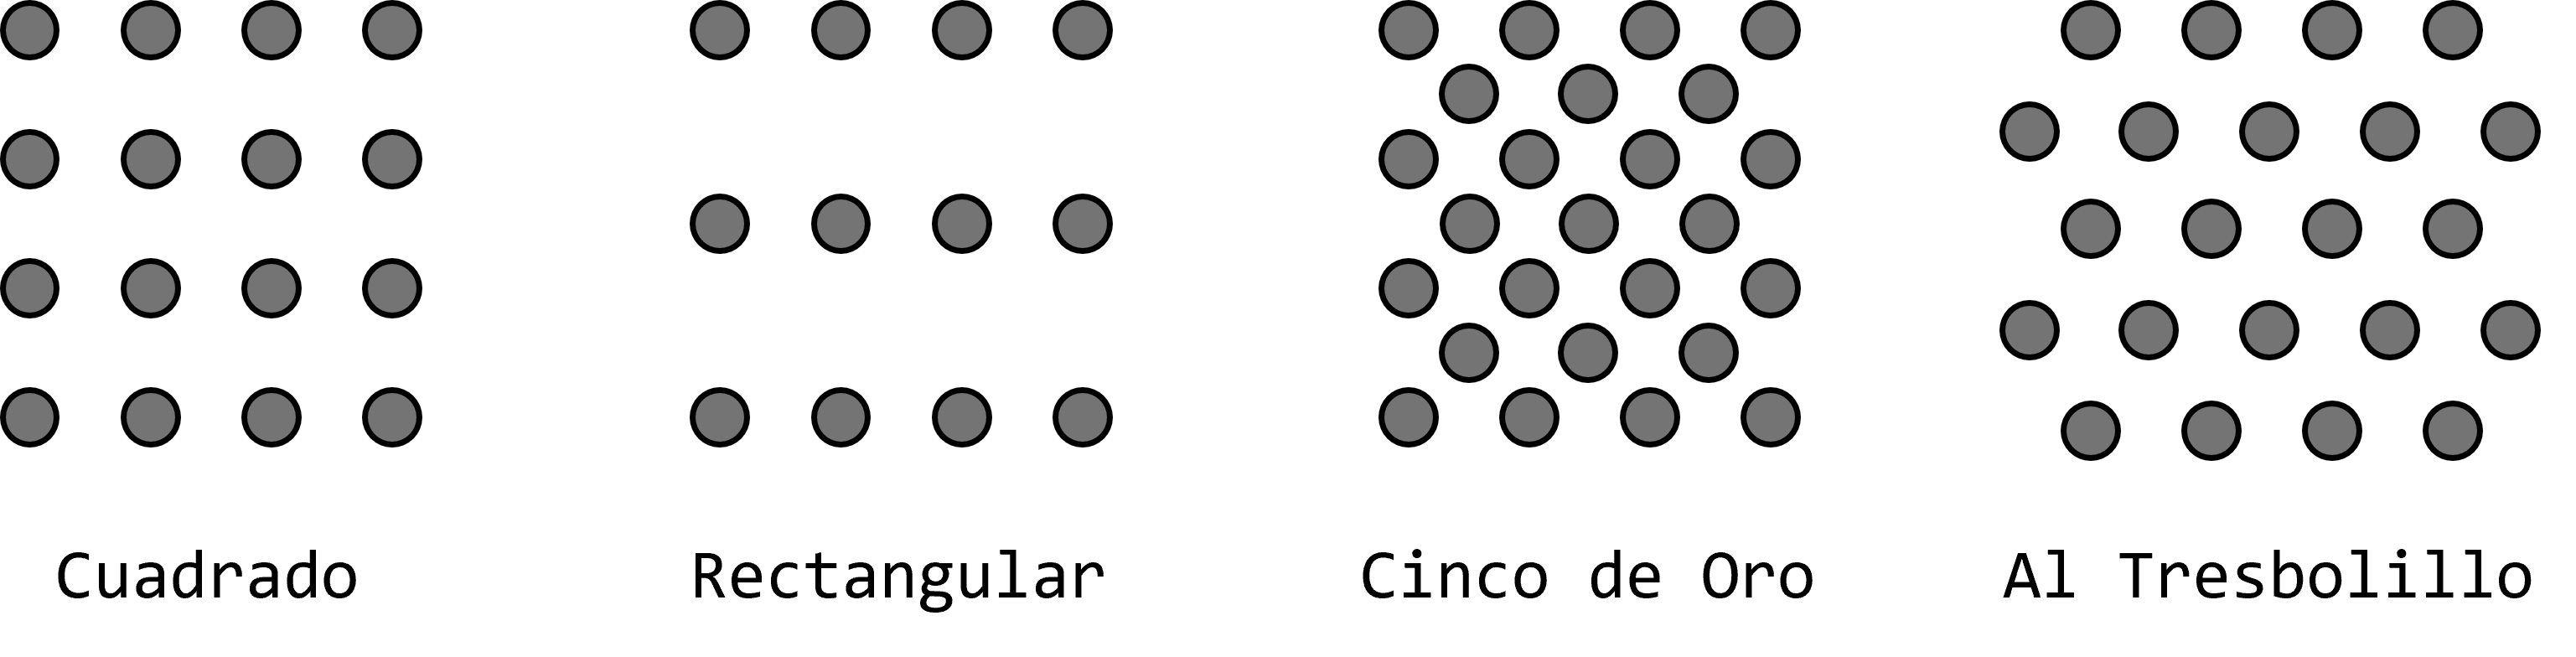
\includegraphics[width=0.8\linewidth]{Sources/figura1.png}
                \caption{Main plantation frames.}\label{fig:MarcosDePlantación}
            \end{figure}
            
            Tres bolillos or trebolillo is one of the most used planting systems today. This is based on planting in the shape of equilateral triangles, where each vertex represents the place where a plant will be planted, this way we ensure that each plant has the same separation with all its neighbors. The reason why this system is so widely used is because it allows better use of the planting space, allowing 17\% (\cite{Anonimo1}) more plants to be planted compared to the rectangular planting method; it also allows better control of erosion and light collection, since the shadow of one tree is not projected directly on others (\cite{Iglesias}).
            To use this system, it is necessary to first decide how much distance there will be between each plant, which depends on its characteristics and the environment. Subsequently, the distance between each groove (rows) is calculated, which is equal to the height of the equilateral triangle (\cite{Guerrero2018}).

            \begin{equation}
                h = d\cos{30}
            \end{equation}
            \\
            where h is the distance between rows and d the distance between each tree. On the other hand, it is possible to know the number of plants that fit in a given space using trigonometry in the following way (\cite{Carbo}):

            \begin{equation}
                n = \frac{A}{d^2 \cos{30}}
            \end{equation}
            where n is the number of plants, A is the area of available land and d is the distance between each plant.



% -------------------------------------- Referencias --------------------------------------
\newpage
\printbibliography[title={References}]



\end{document}